\documentclass[a4paper,11pt]{article}

\usepackage[french]{babel}
\usepackage[T1]{fontenc}
\usepackage[utf8]{inputenc}
\usepackage{graphicx}
\usepackage{hyperref}
%\usepackage{fullpage}

\begin{document}

\title{\textbf{Compte rendu du TP \no 1}\\Changement d'espace couleur}
\author{Thibaut Castanié\\\textit{M2 IMAGINA}}
\date{\today}

\maketitle
\thispagestyle{empty}

\newpage 

\section{Image originale choisie}

\begin{center}
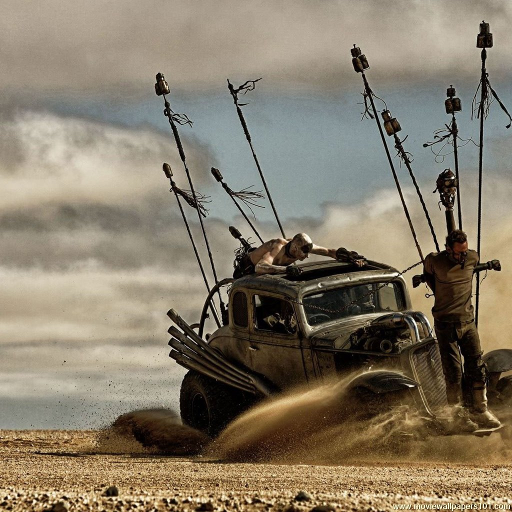
\includegraphics[scale=0.5]{./imgs/madmax.png}\\
\textit{L'image originale utilisée pour le TP}
\end{center}

\newpage

\section{Compression dans l'espace RGB}
\paragraph{} J'ai choisi de réduire la taille des composantes Verte et Bleue. Pour diminuer leur taille, je fait la moyenne de la valeur des pixels dans chaque région de 4x4 de l'image, et je la sauvegarde, dans l'ordre, dans une image deux fois plus petite.

\begin{center}
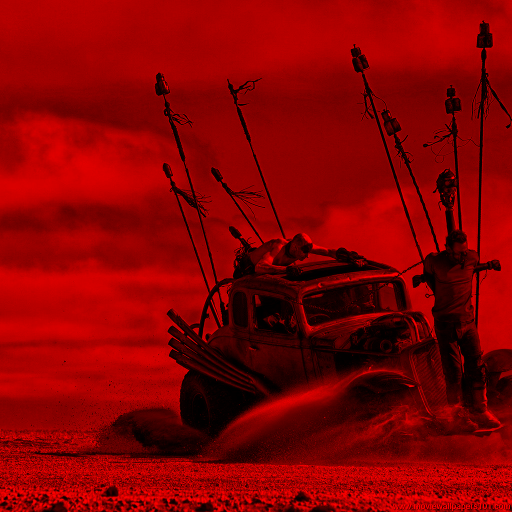
\includegraphics[scale=0.5]{./imgs/madmax2R.png}
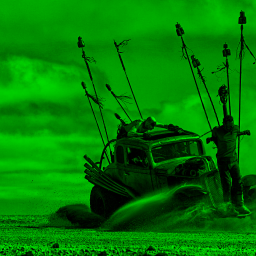
\includegraphics[scale=0.5]{./imgs/madmax2G.png}
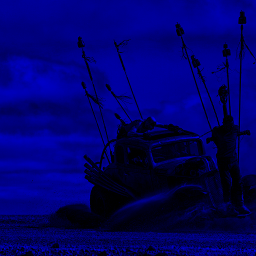
\includegraphics[scale=0.5]{./imgs/madmax2B.png}\\
\textit{La composante Verte et Bleue a été réduite}
\end{center}

\paragraph{} Ensuite on agrandit de nouveau les deux composantes précédentes, en utilisant le même algorithme précédent, mais dans l'autre sens. Pour chaque pixel, on applique sa valeur quatre fois dans la nouvelle image : sur le pixel de gauche, celui du bas et celui en bas à droite.

\begin{center}
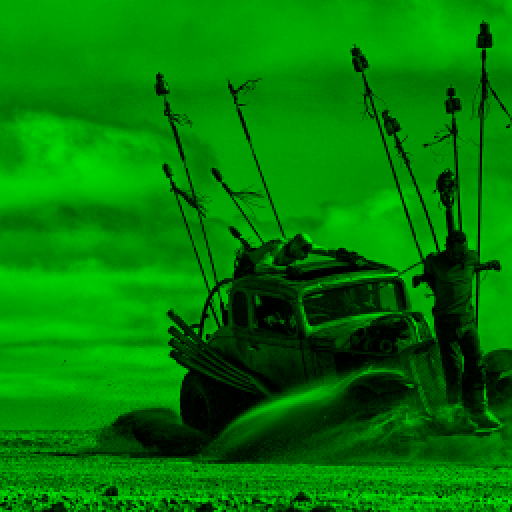
\includegraphics[scale=0.5]{./imgs/madmax3G.png}
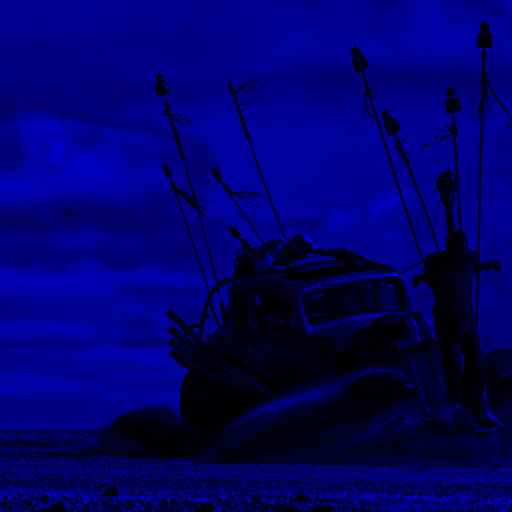
\includegraphics[scale=0.5]{./imgs/madmax3B.png}\\
\textit{La composante Verte et Bleue agrandie}
\end{center}

\paragraph{} Enfin, nous pouvons reconstruire l'image originale en fusionnant les deux composantes ré-échantillonnées avec la composante rouge non modifiée.

\begin{center}
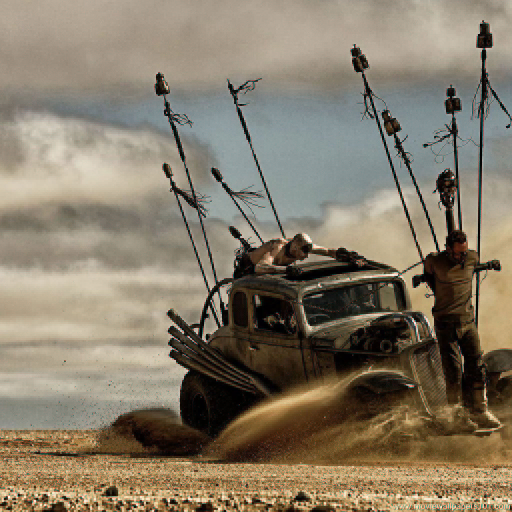
\includegraphics[scale=0.5]{./imgs/madmaxCompRGB.png}\\
\textit{L'image reconstruite}
\end{center}

\paragraph{} Visuellement, on constate une perte de qualité de l'image, et les objets semblent être entourés d'un léger contour rouge.  Nous avons calculé le PSNR (Peak Signal to Noise Ratio) qui permet de calculer la qualité de l'image compressée par rapport à l'image originale.\\
\textbf{> EQM: 1.20079e+08 | PSNR: 32.6639}

\newpage

\section{Compression dans l'espace YCbCr}
Les mêmes opérations ont étés appliquées dans l'espace YCbCr. Cependant, afin d'avoir un aperçu du résultat, j'ai affiché l'image convertie de RGB vers YCbCr, dans l'espace RGB. J'obtiens ainsi les résultats suivants.

\begin{center}
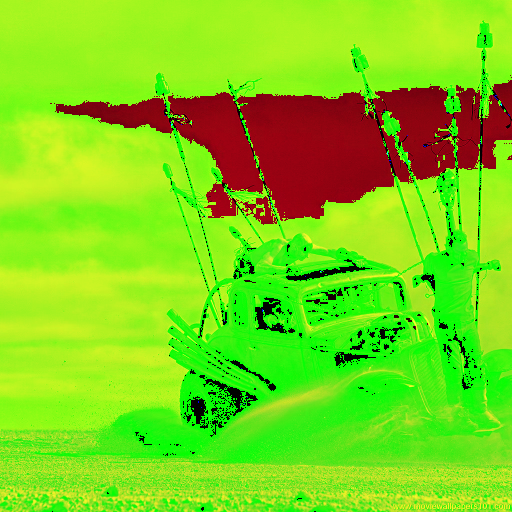
\includegraphics[scale=0.5]{./imgs/madmaxYCbCr.png}\\
\textit{L'image YCbCr affichée dans l'espace RGB}
\end{center}

\begin{center}
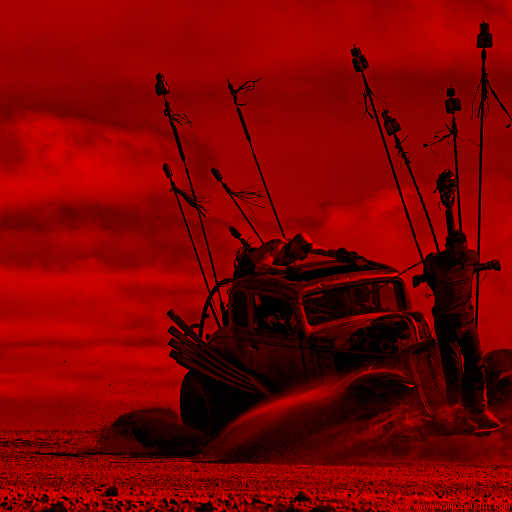
\includegraphics[scale=0.2]{./imgs/madmaxY2R.png}
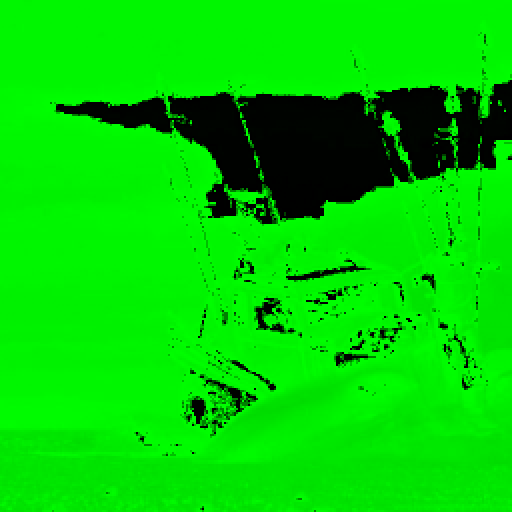
\includegraphics[scale=0.2]{./imgs/madmaxY3G.png}
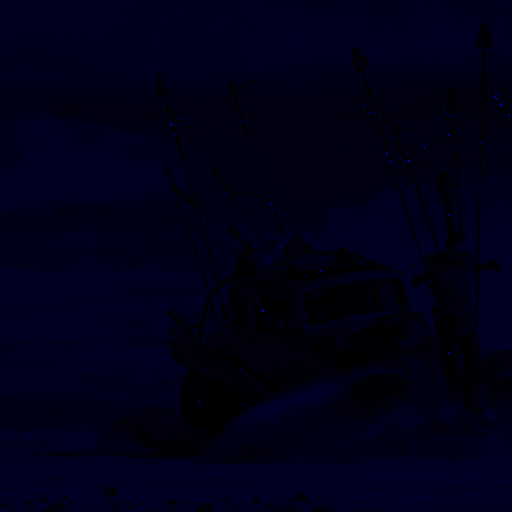
\includegraphics[scale=0.2]{./imgs/madmaxY3B.png}\\
\textit{Les composantes G et B ont étés ré-échantillonnées, réduites puis agrandies}
\end{center}

\begin{center}
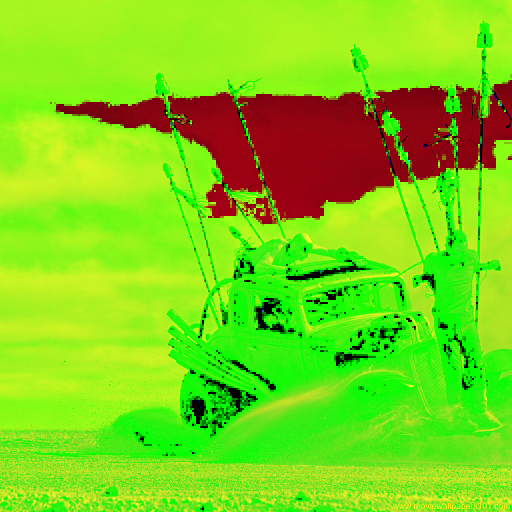
\includegraphics[scale=0.5]{./imgs/madmaxYCompRGB.png}\\
\textit{L'image YCbCr reconstruite}
\end{center}

\paragraph{} \textbf{EQM: 1.35187e+08 | PSNR: 33.1785}

\section{Conclusion}
\paragraph{} Bien que le PSNR obtenu en comparant l'image originale et l'image compressée soit acceptable, le rendu visuel de l'image compressée est médiocre. En effet, on obtient un rendu très pixelisé de l'image, en plus d'avoir un léger contour rouge (la composante non compressée) autour des objets de l'image.

\paragraph{} Une autre approche pour compresser une image serait de prendre les pixels dont la valeur est impaire, et de diminuer leur valeur de 1 pour qu'elle devienne paire. Ainsi, l'image comporterait deux fois moins de couleurs, et cela ne se verrait presque pas à l'oeil nu.

\section*{Annexes - Code}

Code appliquant les opérations du TP : \href{https://github.com/Ooya/M2-IMAGINA/blob/master/Compression/TP1/compressionRGB.cpp}{compressionRGP.cpp}

Code convertissant une image RGB en YCbCr : \href{https://github.com/Ooya/M2-IMAGINA/blob/master/Compression/TP1/convRGBtoYCbCr.cpp}{convertRGBtoYCbCr.cpp}
\end{document}